\begin{figure*}
    \centering
    \begin{minipage}{0.8\textwidth}
    \centering
    \begin{subfigure}{0.3\textwidth}
        \centering 
        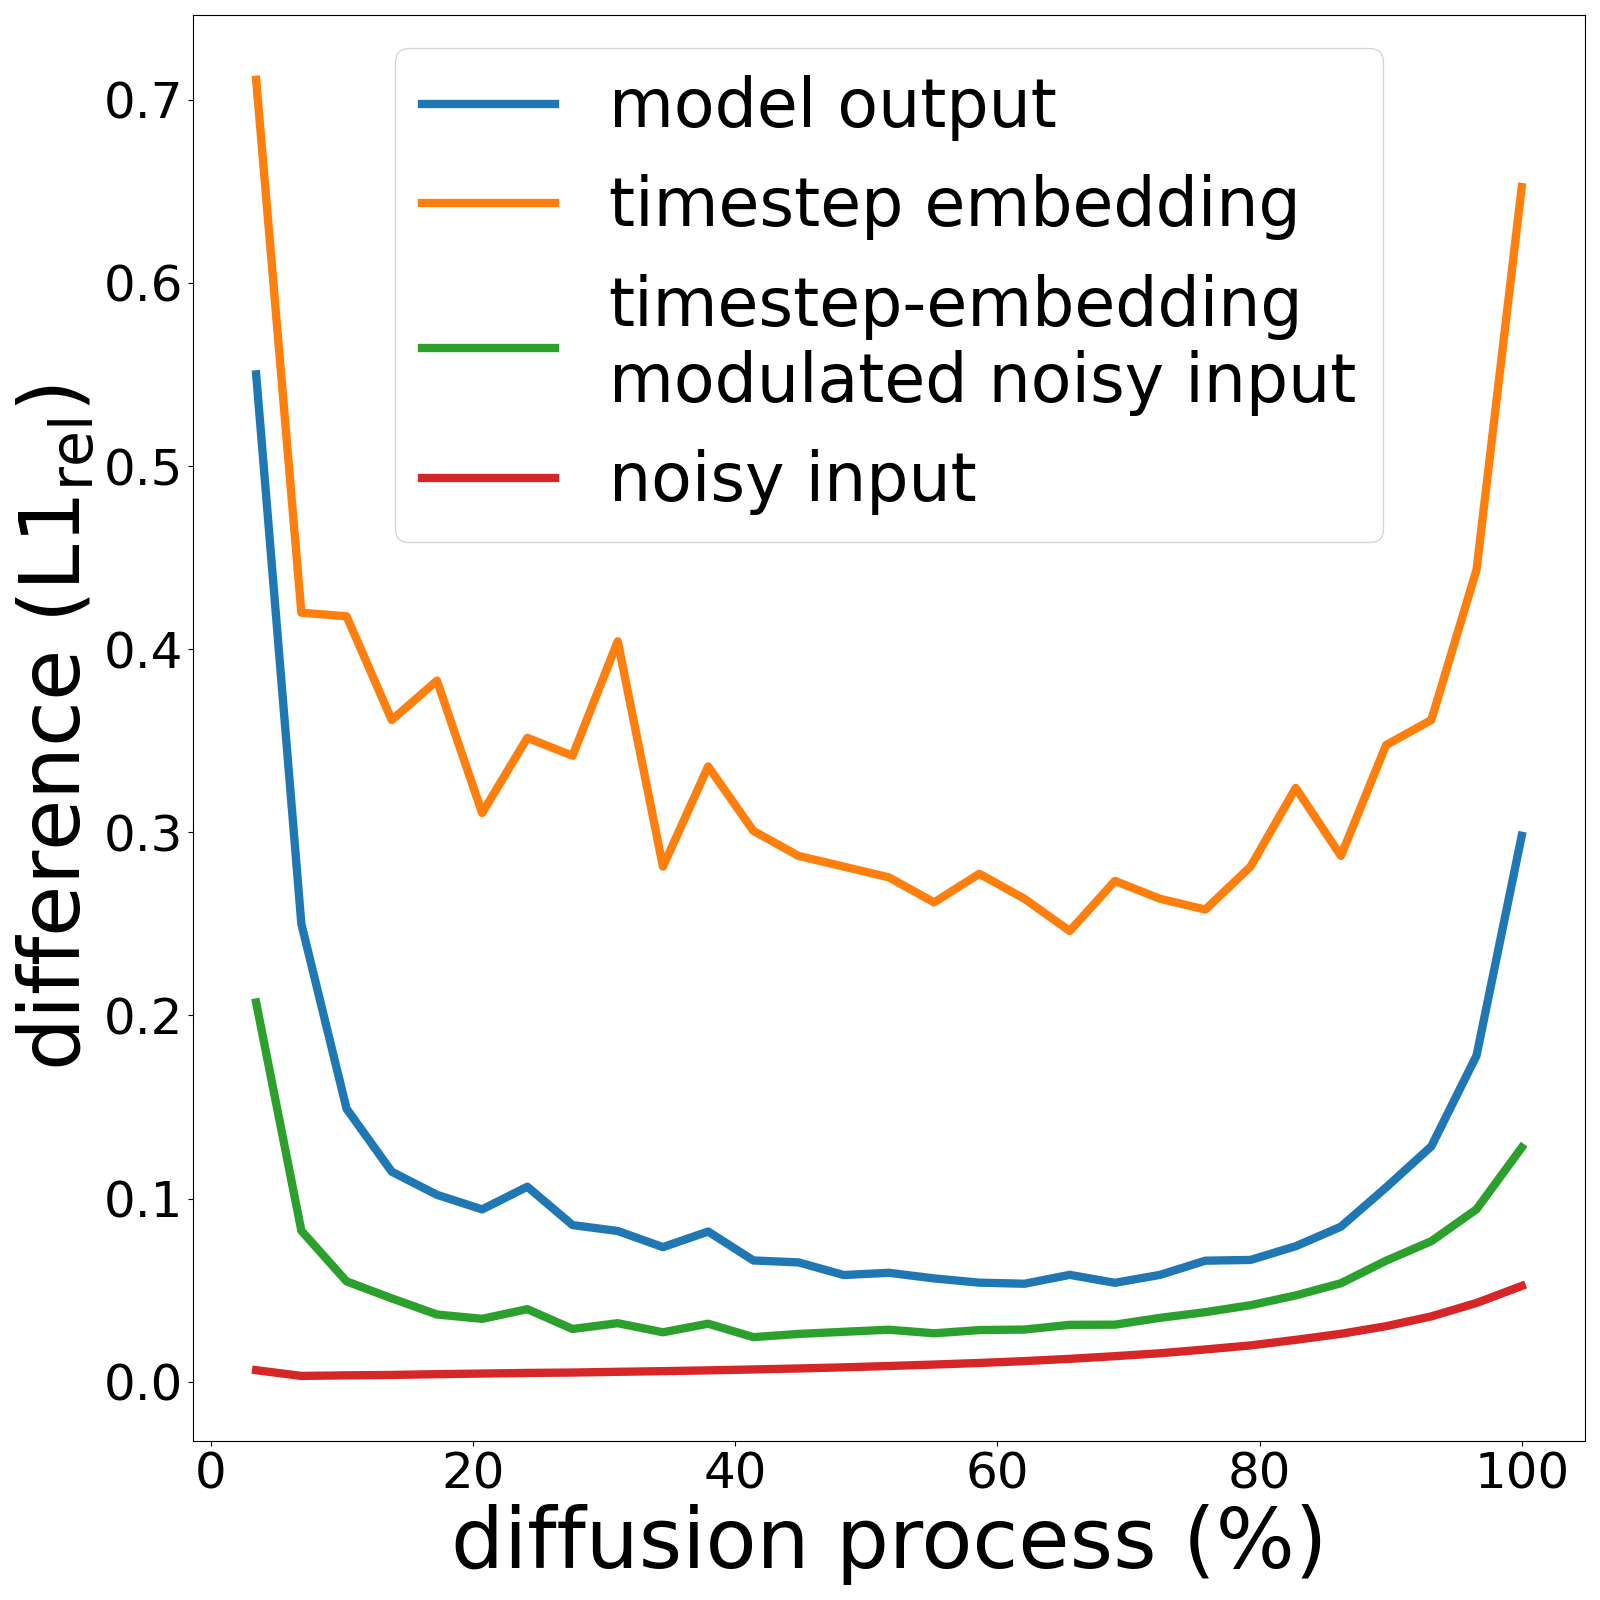
\includegraphics[width=\textwidth]{figs/opensora_inference_difference_crop_5.png}
        \caption{Open Sora}
        % \label{fig:sub1}
    \end{subfigure}
    \hfill
    \begin{subfigure}{0.3\textwidth}
        \centering
        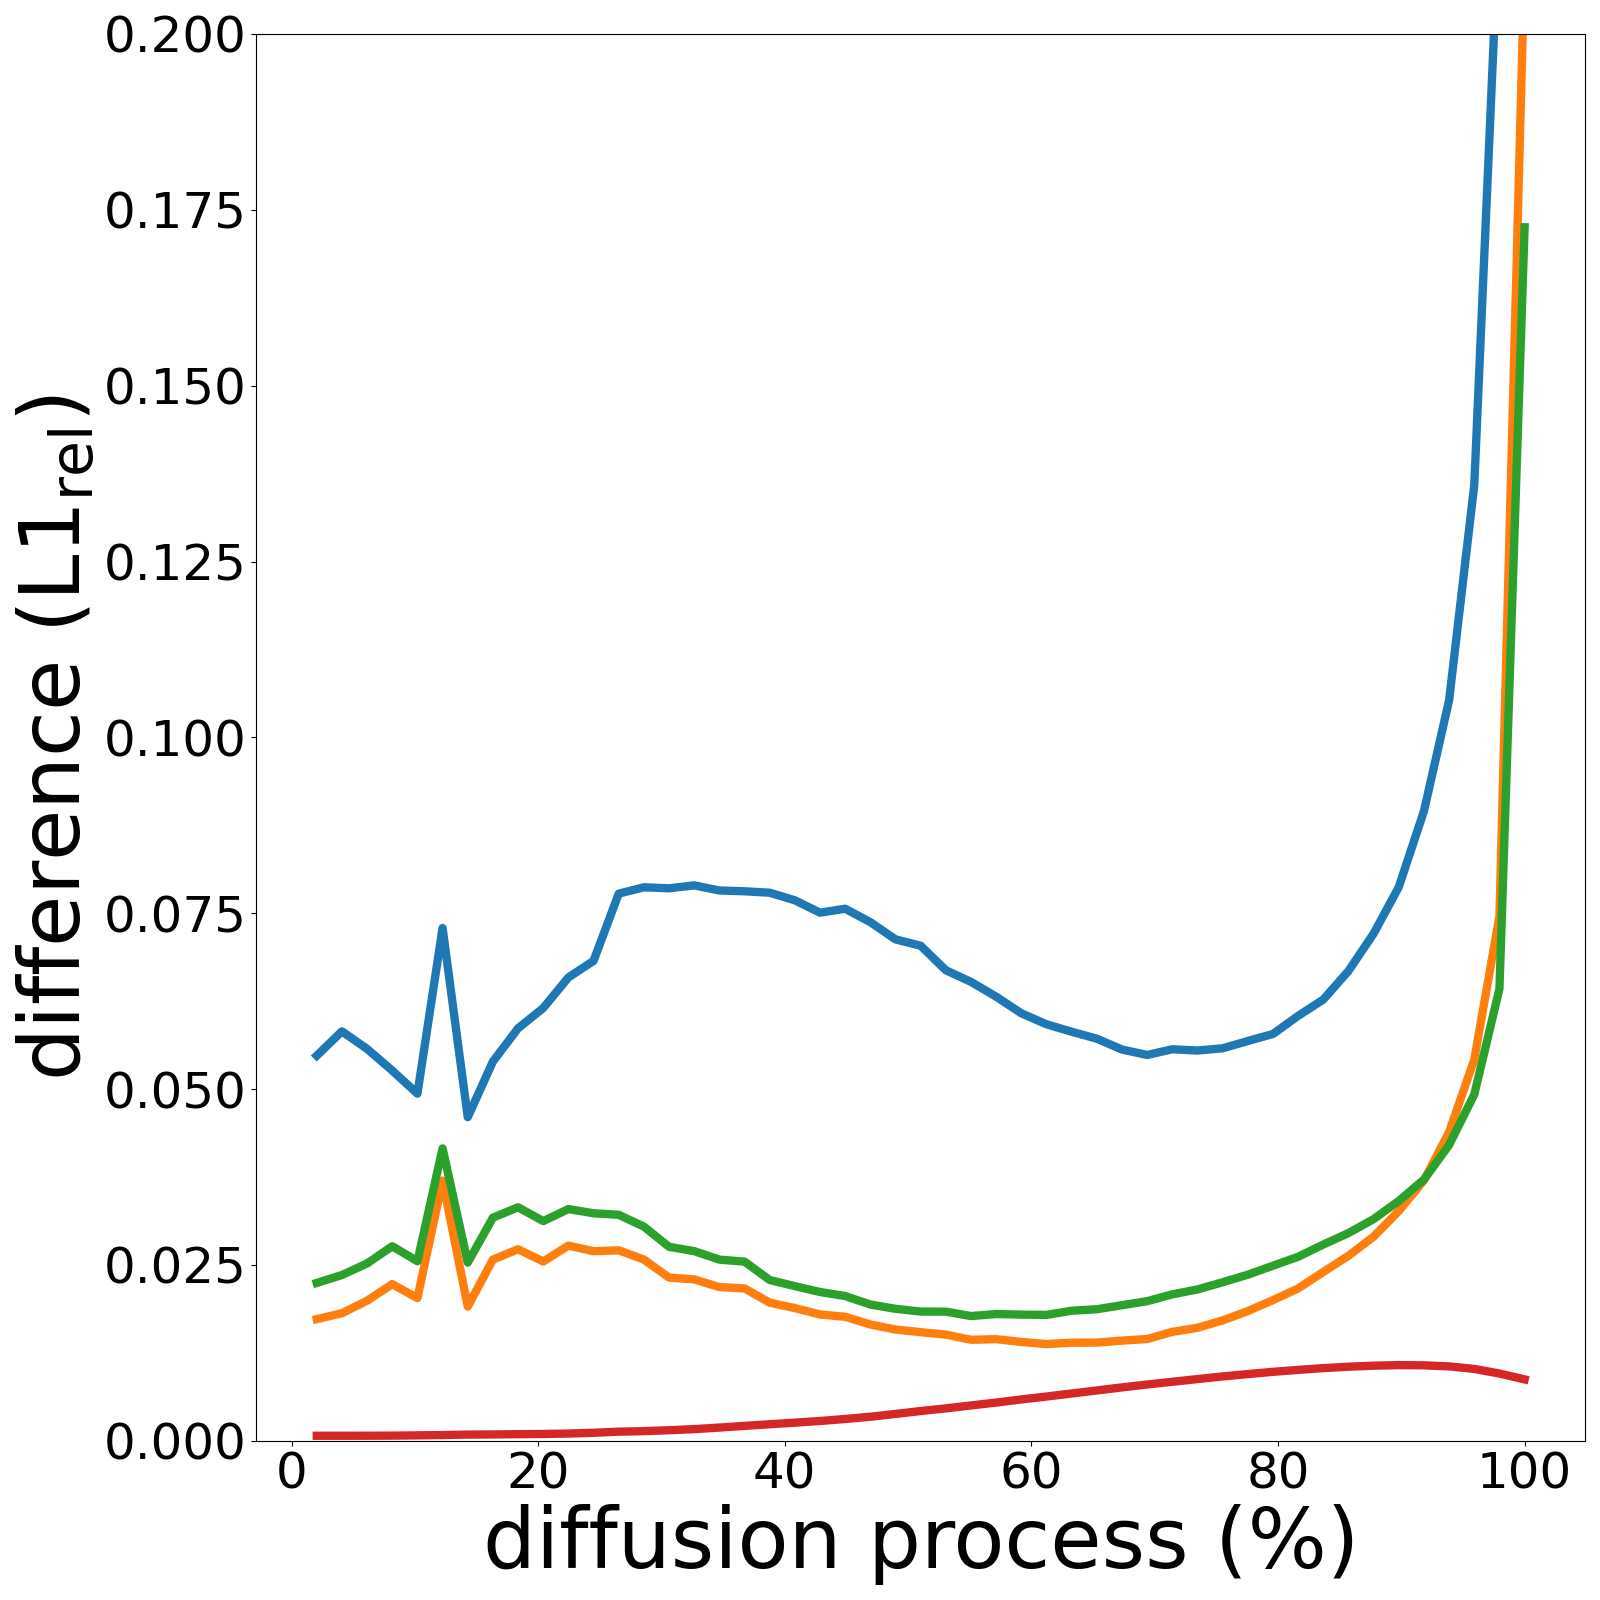
\includegraphics[width=\textwidth]{figs/latte_inference_difference_crop_4.png} 
        \caption{Latte}
        % \label{fig:sub2}
    \end{subfigure}
    \hfill
    \begin{subfigure}{0.3\textwidth}
        \centering
        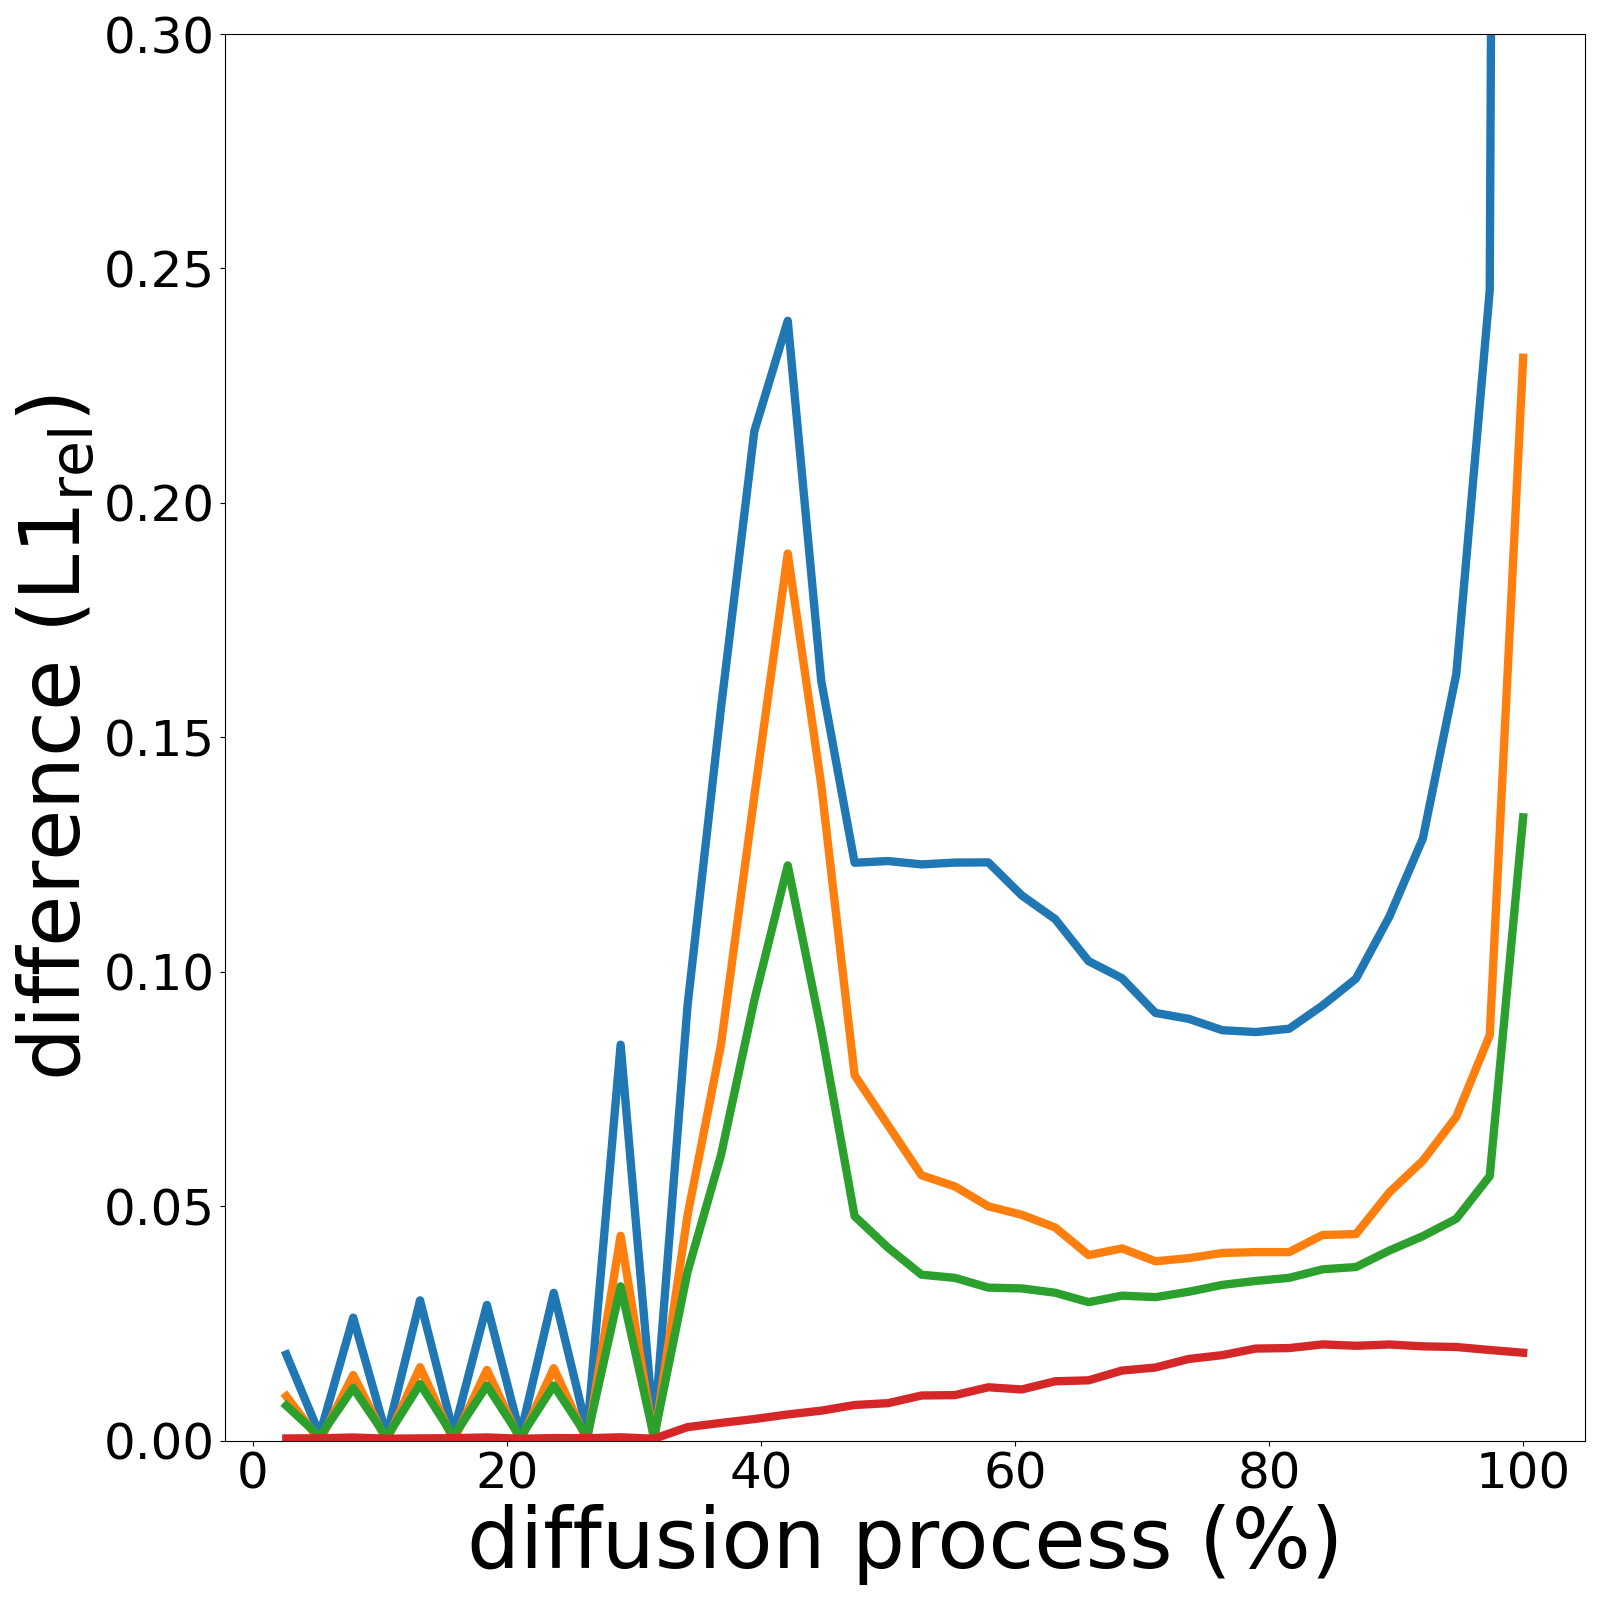
\includegraphics[width=\textwidth]{figs/opensora_plan_inference_difference_crop_4.png} 
        \caption{OpenSora-Plan}
        % \label{fig:sub2}
    \end{subfigure}
    \end{minipage}
    \vspace{-0.2cm}
    \caption{Visualization of input differences and output differences in consecutive timesteps of Open Sora, Latte, and OpenSora-Plan.
    Timestep embedding and Timestep embedding modulated noisy input have strong correlation with model output.}
    \label{fig:difference}
\end{figure*}

\section{Methodology}



\subsection{Preliminaries}
\textbf{Denoising Diffusion Models.} Diffusion models simulate visual generation through a sequence of iterative denoising steps. The core idea is to start with random noise and progressively refine it until it approximates a sample from the target distribution. During the forward diffusion process, Gaussian noise is incrementally added over T steps to a data point $\mathbf{x}_{0}$ sampled from the real distribution $q(\mathbf{x})$:
\begin{equation}
\mathbf{x}_{t}=\sqrt{\alpha_{t}} \mathbf{x}_{t-1}+\sqrt{1-\alpha_{t}} \mathbf{z}_{t} \quad \text { for } \quad t=1, \ldots, T
\end{equation}
where $\alpha_t \in [0,1]$ governs the noise level, and $\mathbf{z}_t \sim \mathcal{N}(\mathbf{0}, \mathbf{I})$ represents Gaussian noise. As $t$ increases, $\mathbf{x}_t$ becomes progressively noisier, ultimately resembling a normal distribution $\mathcal{N}(\mathbf{0}, \mathbf{I})$ when $t=T$. The reverse diffusion process is designed to reconstruct the original data from its noisy counterpart:
\begin{equation}
p_\theta(\mathbf{x}_{t-1} \mid \mathbf{x}_t) = \mathcal{N}(\mathbf{x}_{t-1}; \mu_\theta(\mathbf{x}_t, t), \Sigma_\theta(\mathbf{x}_t, t)),
\end{equation}
where $\mu_\theta$ and $\Sigma_\theta$ are learned parameters defining the mean and covariance.

\begin{figure}
  \centering
    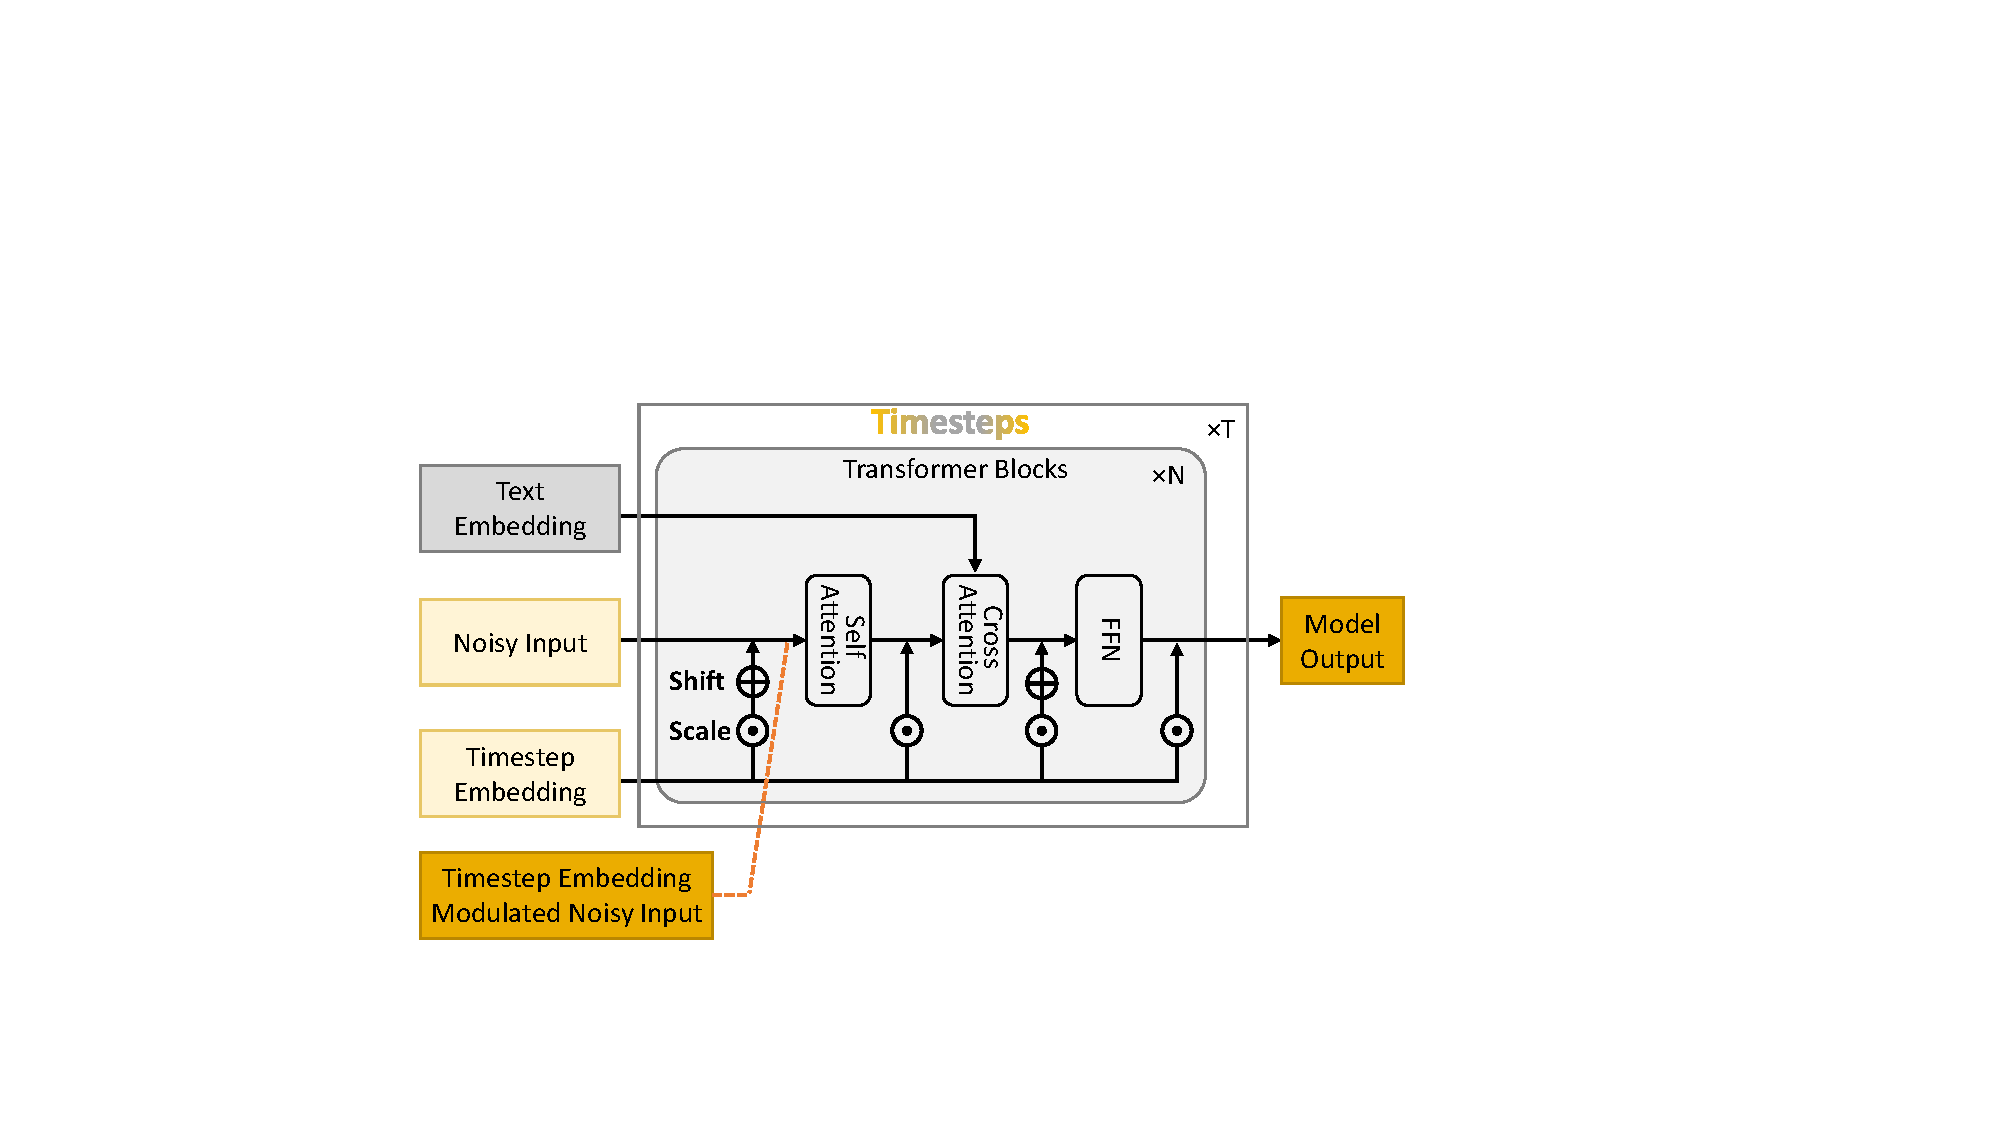
\includegraphics[width=1.0\linewidth]{figs/block.pdf}
  \caption{Diffusion module of the visual generation model with transformer. Normalization layer is omitted for simplicity. Timestep embedding modulates the magnitude of block input and output thus has the potential to indicate the variation of output.}
  \label{fig:block}
\end{figure}




\textbf{Timestep Embedding in Diffusion Models.} 
The diffusion procedures are usually splitted to one thousand timesteps during training phase and dozens of timesteps during inference phase. Timestep defines the strength of noise to be added or removed in the diffusion procedures, which is an important input of the diffusion model. Specifically, the scalar timestep $t$ is firstly transformed to timestep embedding through sinusoidal embedding and multilayer perception module:
\begin{equation}
\mathbf{T}_{t} = MLP(sinusoidal(t))\quad \text { for } \quad t=1, \ldots, T.
\end{equation}
Timestep embedding then modulates the input and output of the Self Attention Layer and Feed Forward Network (FFN) in each Transformer block, as shown in Fig.\ref{fig:block}. Thus, timestep embedding can significantly affect the magnitude of the model output.


\begin{figure*}
    \centering
    \begin{minipage}{0.8\textwidth}
    \centering
    \begin{subfigure}{0.3\textwidth}
        \centering 
        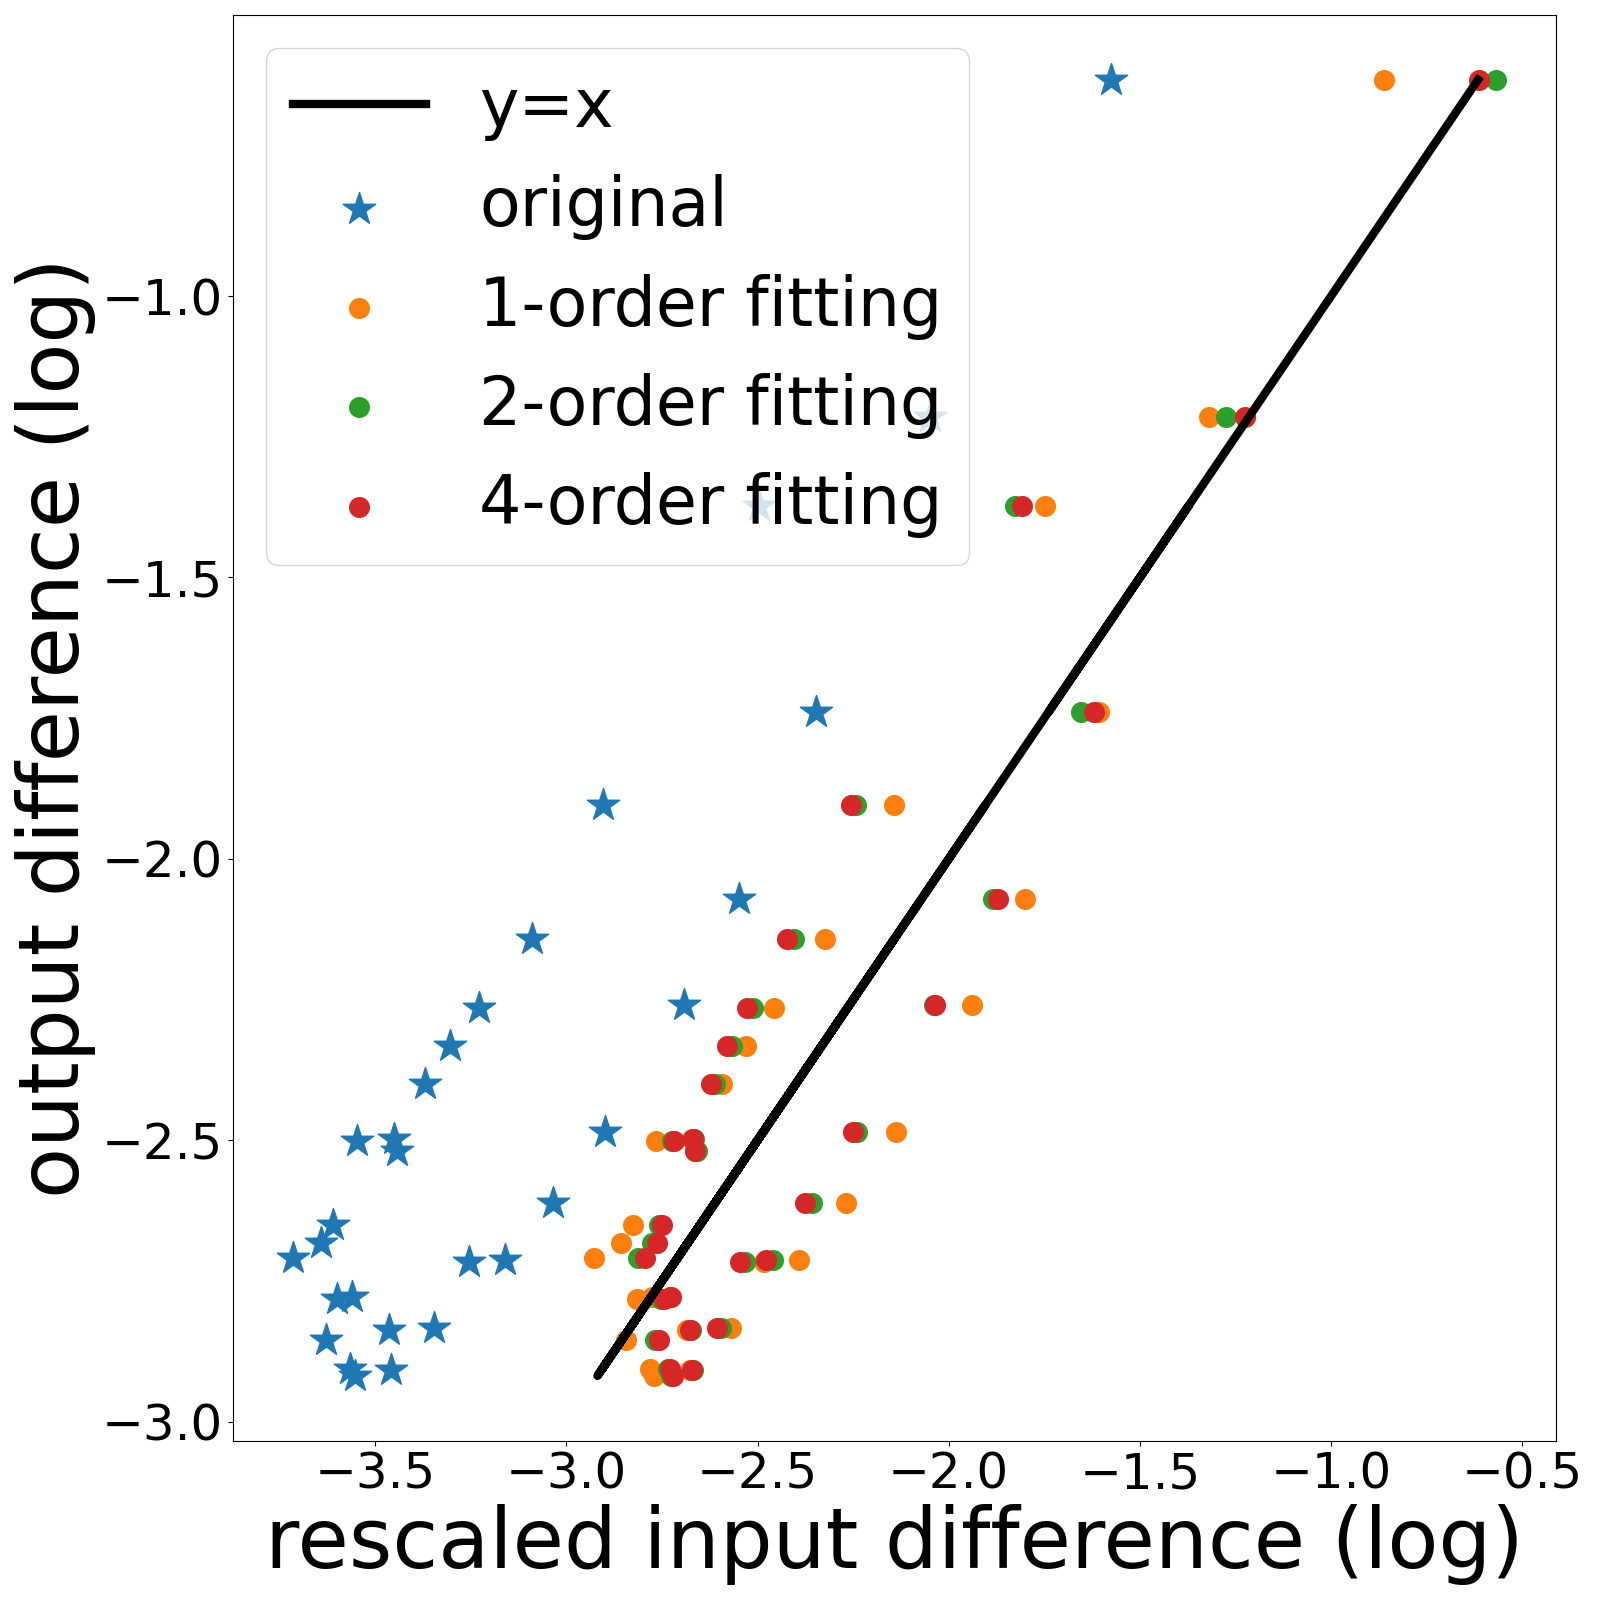
\includegraphics[width=\textwidth]{figs/opensora_inference_fit_log_3.png} 
        \caption{Open Sora}
        % \label{fig:sub1}
    \end{subfigure}
    \hfill
    \begin{subfigure}{0.3\textwidth}
        \centering
        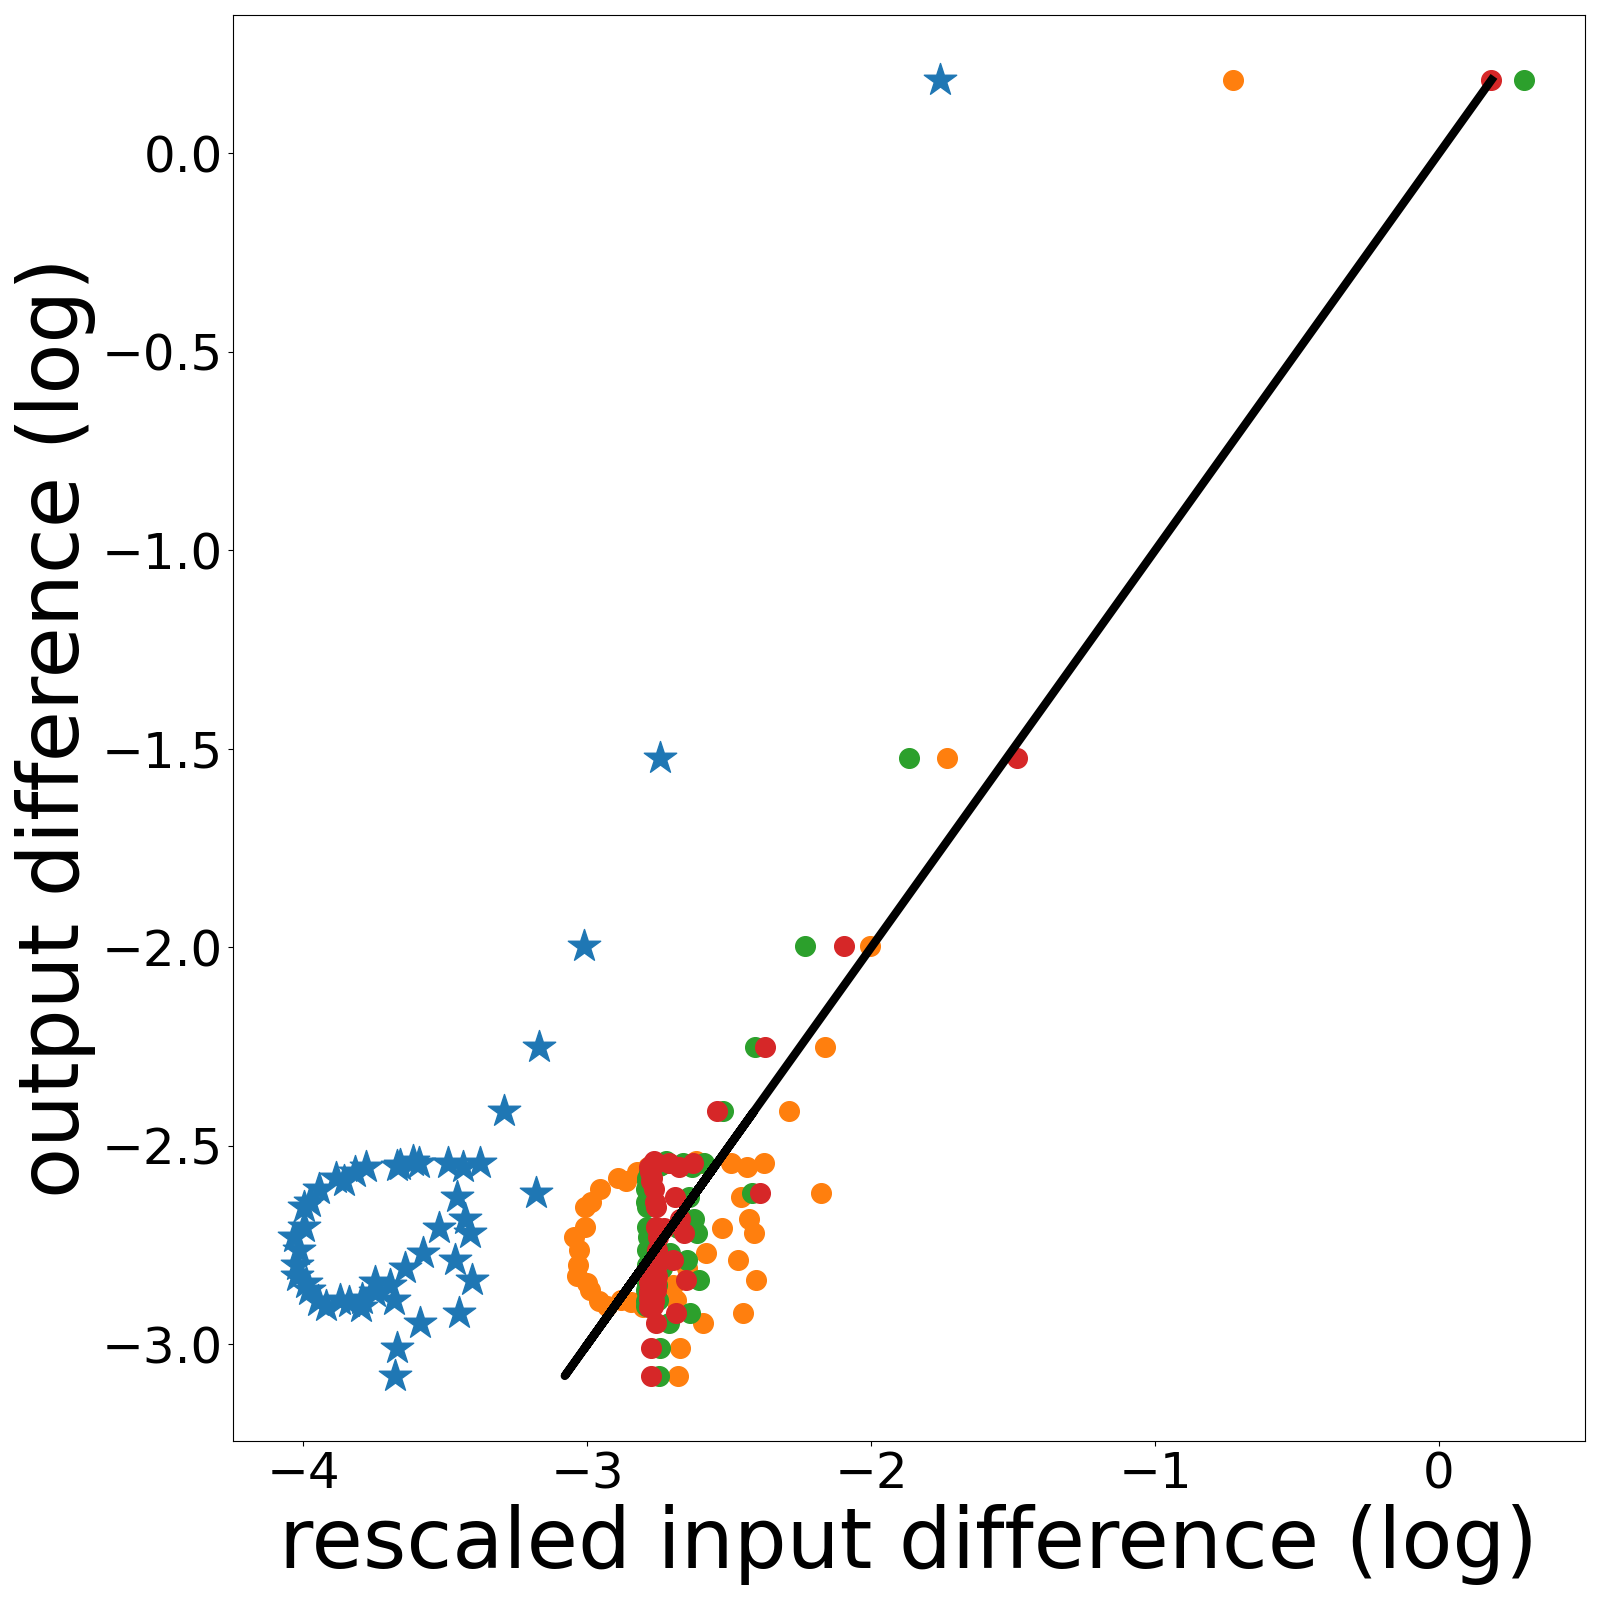
\includegraphics[width=\textwidth]{figs/latte_inference_fit_log_3.png} 
        \caption{Latte}
        % \label{fig:sub2}
    \end{subfigure}
    \hfill
    \begin{subfigure}{0.3\textwidth}
        \centering
        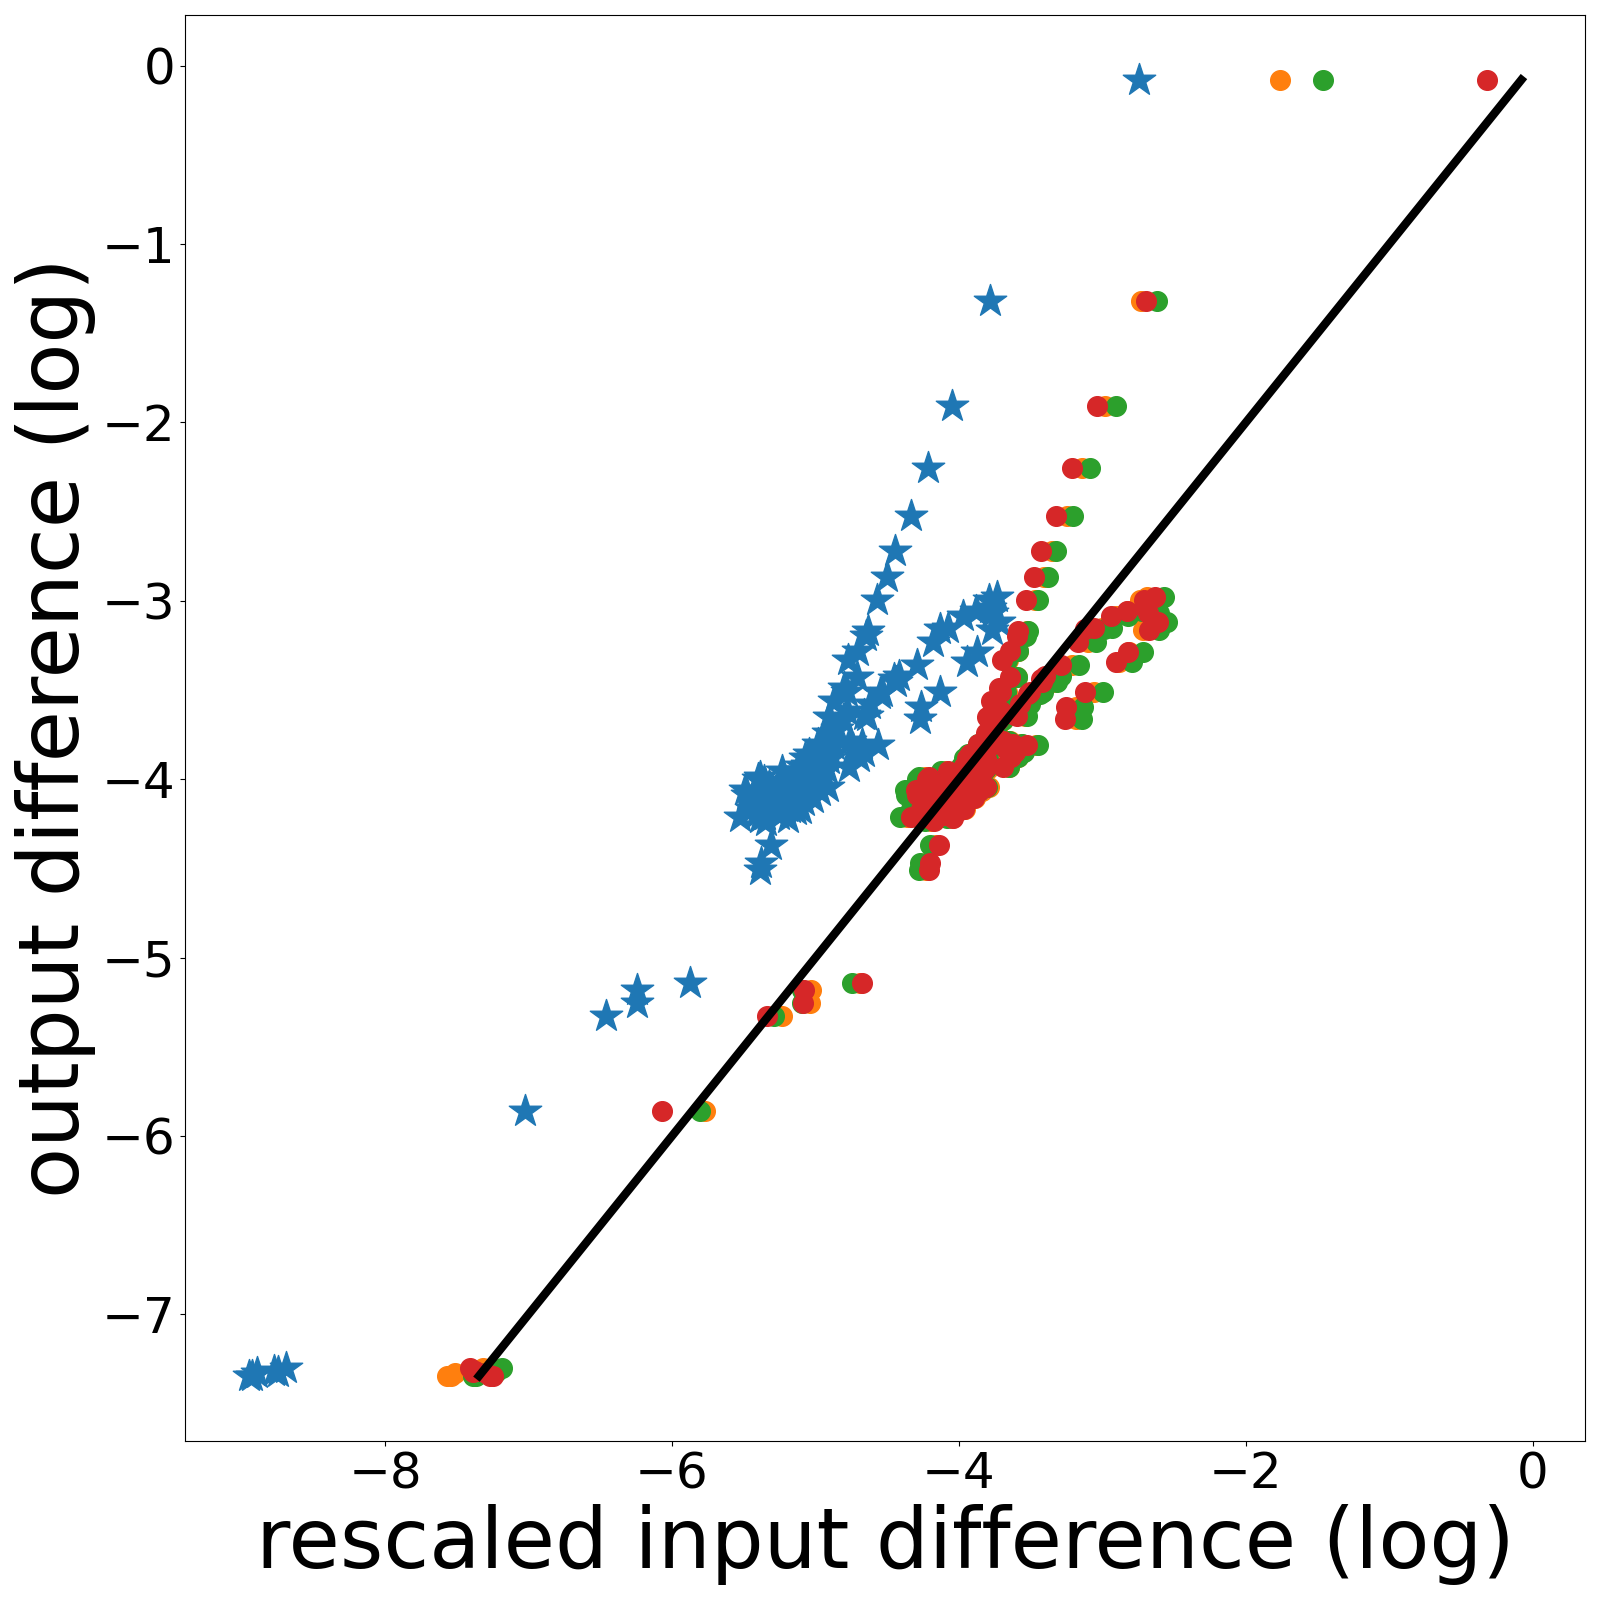
\includegraphics[width=\textwidth]{figs/opensora_plan_inference_fit_log_3.png}
        \caption{OpenSora-Plan}
        % \label{fig:sub2}
    \end{subfigure}
    \end{minipage}
    \vspace{-0.2cm}
    \caption{Visualization of corelation of input differences and output differences in consecutive timesteps of Open Sora, Latte, and OpenSora-Plan. 
    The original data points deviate a lot from the linear corelation. Polynomial fitting reduces the gap.}
    \label{fig:fitting}
\end{figure*}

\begin{figure}
  \centering
    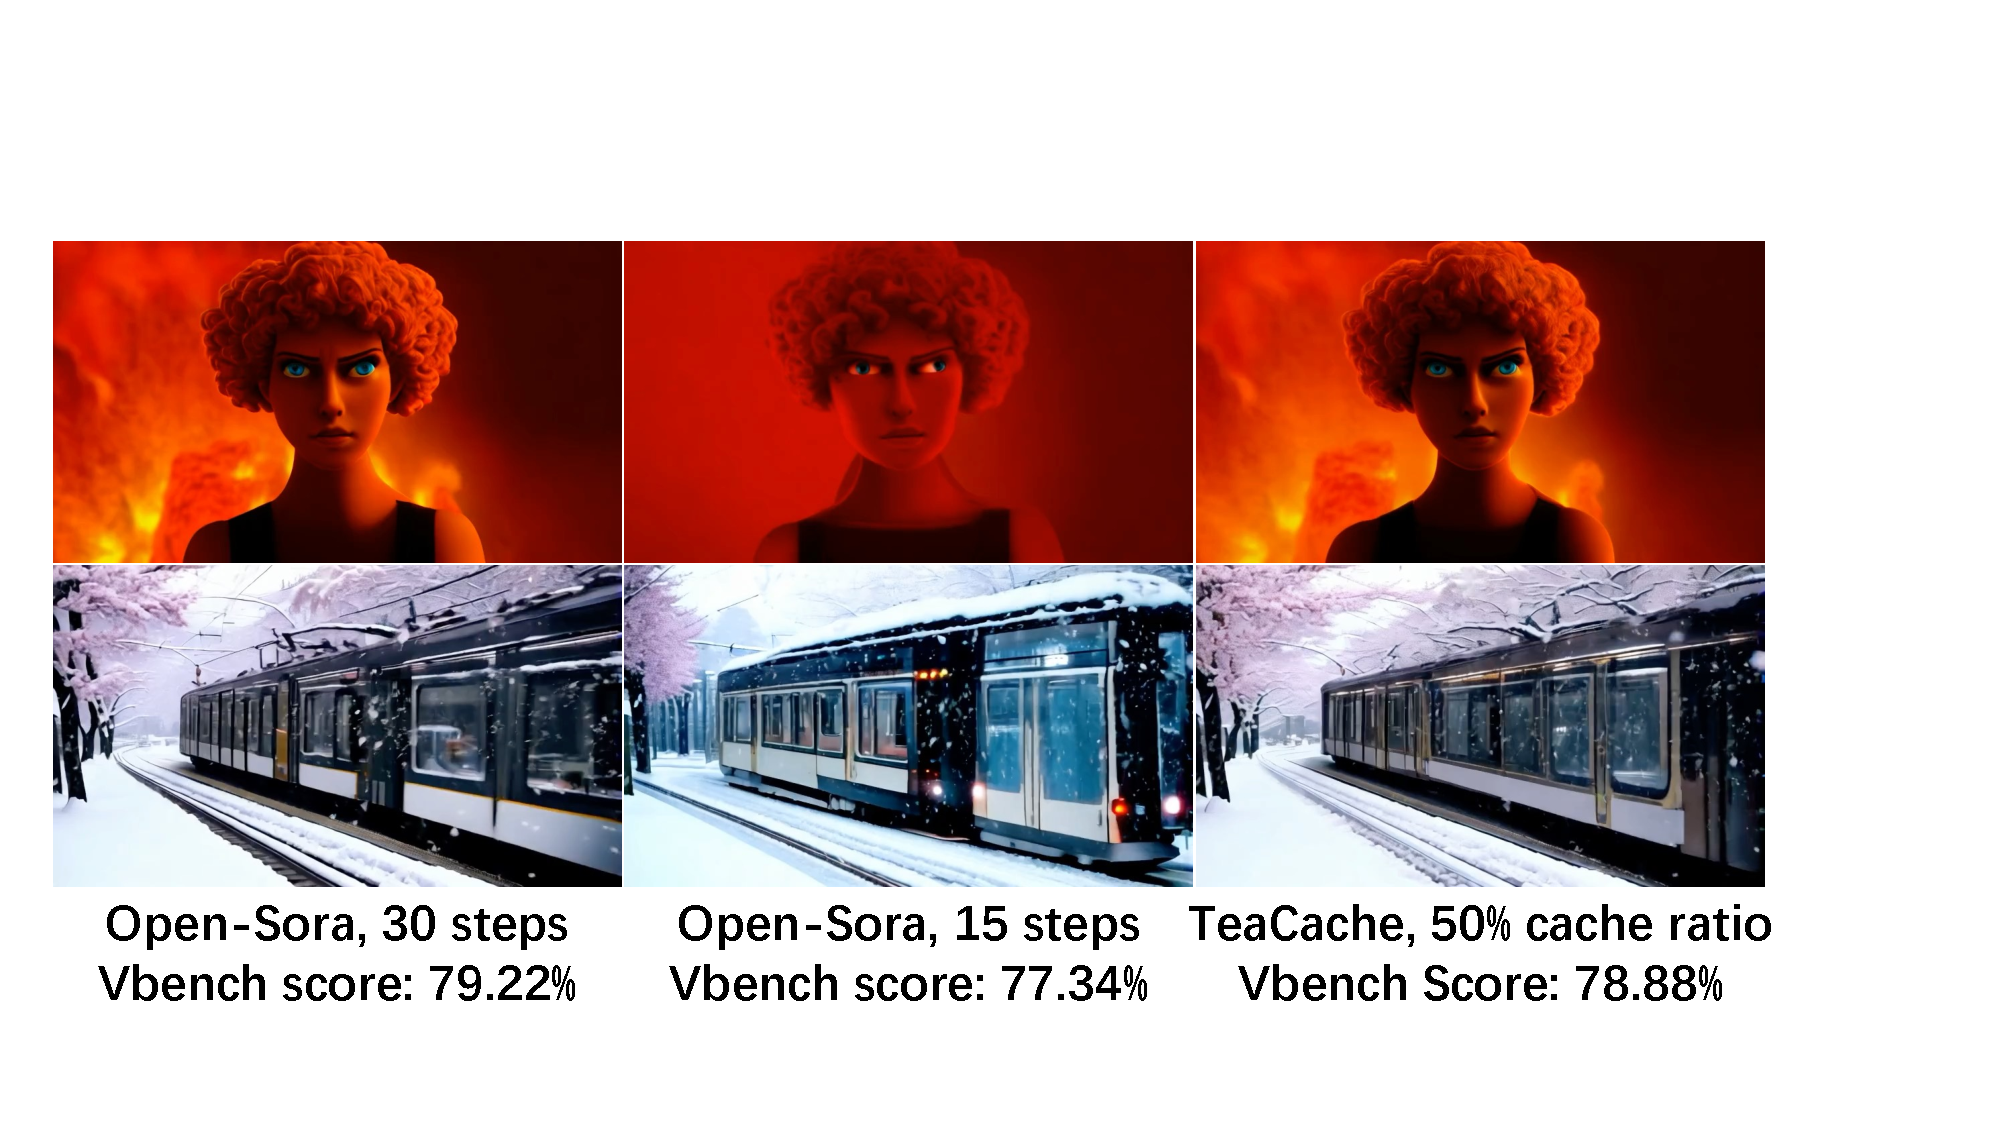
\includegraphics[width=1.0\linewidth]{figs/reducing_steps.pdf}
  \caption{Caching Mechanism \textit{v.s.} Reducing Timesteps. Reducing inference timesteps suffers from deteriorated visual quality while TeaCache maintains visual quality.}
  \label{fig:few timestep}
\end{figure}

\subsection{Analysis}
To investigate the correlation between model output and input, we perform an in-depth analysis of their behaviors during the diffusion process. 

\textbf{Model outputs:} Ideally, if we could obtain the model outputs in advance, we could directly measure the difference between outputs at adjacent timesteps and decide whether to cache the outputs based on their difference. 
Following ~\cite{wimbauer2024cache}, we use the relative L1 distance as our metric. For instance, the relative L1 distance $\text{L1}_{\text{rel}}(\mathbf{O}, t)$ for output embedding $\mathbf{O}_t$ at timestep $t$ is calculated as follows:
\begin{equation}
\text{L1}_{\text{rel}}(\mathbf{O}, t) = \frac{\|\mathbf{O}_t - \mathbf{O}_{t+1}\|_1}{\|\mathbf{O}_{t+1}\|_1}
\label{eq:difference_measurement}
\end{equation}
where a large $\text{L1}_{\text{rel}}(\mathbf{O}, t)$ indicates that $\mathbf{O}_t$ is informative relative to $\mathbf{O}_{t+1}$ and should be cached; otherwise, a small $\text{L1}_{\text{rel}}(\mathbf{O}, t)$ indicates that $\mathbf{O}_{t+1}$ and $\mathbf{O}_t$ are similar to each other and therefore $\mathbf{O}_{t+1}$ could be reused to replace $\mathbf{O}_{t}$. Therefore, Eq.~\ref{eq:difference_measurement} can be used to define a criterion for determining whether the model outputs should be cached.

However, in most cases, the model outputs cannot be obtained in advance, making the above approach infeasible. To address this issue, an intuitive idea is that if we can efficiently estimate the difference of the model outputs, we can leverage it to design a caching strategy. Fortunately, it is well-known that the model inputs and outputs are strongly correlated. Based on this insight, we analyzed the model inputs and conducted detailed experiments to investigate their correlation with the model outputs.

\textbf{Model inputs:} We consider the inputs of diffusion model: text embedding, timestep embedding, and noisy input, as shown in Fig.~\ref{fig:block}. Since the text embedding remains constant throughout the diffusion process, it cannot be used to measure the difference of inputs across timestep. Therefore, text embedding is excluded from analysis. As for the timestep embedding, it changes as timesteps progress but is independent of the noisy input and text embedding, making it difficult to fully reflect the information of the input. The noisy input, on the other hand, is gradually updated during the denoising process and contains information from the text embedding, but it is not sensitive to timesteps. To comprehensively represent the model inputs and ensure their correlation with the outputs, we ultimately utilized the timestep embedding modulated noisy input at the Transformer’s input stage as the final input embedding, as illustrated in the Fig.~\ref{fig:block}.

\textbf{Experimental analysis:}
To derive a robust conclusion, we make analysis using the metric defined in Eq.~\ref{eq:difference_measurement} to compute the difference of model inputs and outputs on three distinct video generation models: Open Sora~\cite{Open-Sora}, Latte~\cite{ma2024latte}, and OpenSora Plan~\cite{Open-Sora-Plan}. As illustrated in Fig.~\ref{fig:difference}, the difference of outputs exhibit distinct patterns across various models. In Open Sora, the pattern forms a 'U' shape, whereas in Latte and OpenSora-Plan, it resembles a horizontally flipped 'L'. Additionally, OpenSora-Plan features multiple peaks because its scheduler samples certain timesteps twice. The noisy input across consecutive timesteps changes minimally and shows little correlation with the model output. In contrast, both the timestep embedding and the timestep embedding modulated noisy input demonstrate a strong correlation with the model output. Given that the timestep embedding modulated noisy inputs exhibits superior generation capabilities (\eg, in Open Sora) and effectively leverages the dynamics of input, we select it as the indicator to determine whether the model output at the current step is similar to that of the previous timestep.


\subsection{TeaCache}
As illustrated in Fig.~\ref{fig:difference}, adjacent timesteps conduct redundant computations where model outputs exhibit minimal change. To minimize these redundancies and accelerate inference, we propose the Timestep Embedding Aware Cache (TeaCache). Rather than computing new outputs at each timestep, we reuse cached outputs from previous timesteps. Our caching technique can be applied to nearly all recent diffusion models based on Transformers.

\textbf{Naive Caching Strategy.} To determine whether to reuse the cached model output from a previous timestep, we employ the accumulated relative L1 distance as an indicator. 
\begin{equation}
\sum_{t=t_a}^{t_b-1} \text{L1}_{\text{rel}}(\mathbf{F}, t) \leq \delta < \sum_{t=t_a}^{t_b} \text{L1}_{\text{rel}}(\mathbf{F}, t)
\end{equation}
where $\text{L1}_{\text{rel}}$ is defined in Eq.~\ref{eq:difference_measurement}. $F$ can be timestep embedding or timestep embedding modulated noisy inputs and $\delta$ is the caching threshold. Specifically, after computing the model output at timestep $t_a$ and caching it, we accumulate the relative L1 distance $\sum_{t=t_a}^{t_b-1} \text{L1}_{\text{rel}}(\mathbf{F}, t)$ for subsequent timesteps. If, at timestep $t_b$ ($>t_a$), $\sum_{t=t_a}^{t_b-1} \text{L1}_{\text{rel}}(\mathbf{F}, t)$ is less than the caching threshold $\delta$, we reuse the cached model output; otherwise, we compute the new model output and set the accumulated relative L1 distance to zero.
A smaller threshold $\delta$ results in more frequent refreshing of cached outputs, while a larger threshold speeds up visual generation but may adversely affect image appearance. The threshold $\delta$ should be chosen to enhance inference speed without compromising visual quality.

\textbf{Rescaled Caching Strategy.} Although timestep embedding modulated noisy inputs exhibit a strong correlation with model outputs, the differences in consecutive timesteps are inconsistent. Directly using the difference of timestep embedding-modulated noisy input to estimate model output difference leads to a scaling bias. Such bias may cause suboptimal timestep selection. Considering that these differences are scalars, we apply simple polynomial fitting to rescale them to reduce the bias. The polynomial fitting is then performed between model inputs (timestep embedding modulated noisy inputs) and outputs, which is formulated as 
\begin{equation}
    y = f(x) = a_0 + a_1 x + a_2 x^2 + \cdots + a_n x^n,
\end{equation}
where $y$ represents estimated difference of model output and $x$ signifies the difference of timestep embedding-modulated noisy inputs. This can be efficiently solved using the \textit{poly1d} function from the numpy package.
With polynomial fitting, the rescaled difference in timestep embedding-modulated noisy inputs better estimates model output difference, as shown in Fig.~\ref{fig:fitting}. The final caching indicator is formulated as
\begin{equation}
\sum_{t=t_a}^{t_b-1} f(\text{L1}_{\text{rel}}(\mathbf{F}, t)) \leq \delta < \sum_{t=t_a}^{t_b} f(\text{L1}_{\text{rel}}(\mathbf{F}, t))
\end{equation}




\begin{table*}[]
    \centering
    \caption{Quantitative evaluation of inference efficiency and visual quality in video generation models. TeaCache consistently achieves superior efficiency and better visual quality across different base models, sampling schedulers, video resolutions, and lengths.
    }
    \label{tab: main}
    \begin{tabular}{c|ccc|cccc}
        \toprule
        \multirow{2}{*}{\textbf{Method}} & \multicolumn{3}{c|}{\textbf{Efficiency}} & \multicolumn{4}{c}{\textbf{Visual Quality}} \\ \cline{2-8}
        % \hline
         & \textbf{FLOPs (P) $\downarrow$} & \textbf{Speedup $\uparrow$} & \textbf{Latency (s) $\downarrow$} & \textbf{VBench $\uparrow$} & \textbf{LPIPS $\downarrow$} & \textbf{SSIM $\uparrow$} & \textbf{PSNR $\uparrow$} \\

         \hline
        \hline
        \multicolumn{8}{c}{\textbf{Latte} (16 frames, 512$\times$512)} \\
        \hline
        \rowcolor[gray]{0.9} Latte $(T = 50)$ & 3.36 & 1$\times$ & 26.90 & 77.40\% & - & - & - \\
        $\Delta$-DiT~\cite{chen2024delta} & 3.36 & 1.02$\times$ & - & 52.00\% & 0.8513 & 0.1078 & 8.65 \\
        T-GATE~\cite{zhang2024cross} & 2.99 & 1.13$\times$ & - & 75.42\% & 0.2612 & 0.6927 & 19.55 \\
        PAB-slow~\cite{zhao2024real} & 2.70 & 1.21$\times$ & 22.16  &76.32\% & 0.2669 & 0.7014 &  19.71 \\
        PAB-fast~\cite{zhao2024real} & 2.52 & 1.34$\times$ & 19.98 & 73.13\% & 0.3903 & 0.6421 &  17.16 \\
        \hline
        TeaCache-slow & 1.86  &1.86 $\times$ & 14.46 & \textbf{77.40}\% & \textbf{0.1901} & \textbf{0.7786} &\textbf{22.09}  \\
        TeaCache-fast & \textbf{1.12}  &\textbf{3.28} $\times$ & \textbf{8.20} & 76.69\% & 0.3133 & 0.6678 &18.62  \\


        
        \hline
        \hline
        \multicolumn{8}{c}{\textbf{Open-Sora 1.2} (51 frames, 480P)} \\
        \hline
        \rowcolor[gray]{0.9} Open-Sora 1.2 $(T = 30)$ & 3.15 & 1$\times$ & 44.56 & 79.22\% & - & - & - \\
        $\Delta$-DiT~\cite{chen2024delta} & 3.09 & 1.03$\times$ & - & 78.21\% & 0.5692 & 0.4811 & 11.91 \\
        T-GATE~\cite{zhang2024cross} & 2.75 & 1.19$\times$ & - & 77.61\% & 0.3495 & 0.6760 & 15.50 \\
        PAB-slow~\cite{zhao2024real} & 2.55 & 1.33$\times$ & 33.40  & 77.64\% & 0.1471 & 0.8405 &  \textbf{24.50} \\
        PAB-fast~\cite{zhao2024real} & 2.50 & 1.40$\times$ & 31.85 & 76.95\% & 0.1743 & 0.8220 &  23.58 \\
        \hline
        TeaCache-slow & 2.40 & 1.55$\times$ & 28.78 & \textbf{79.28}\% & \textbf{0.1316} & \textbf{0.8415} &23.62  \\
        TeaCache-fast & \textbf{1.64} & \textbf{2.25}$\times$ & \textbf{19.84} & 78.48\% & 0.2511 & 0.7477 & 19.10 \\

        

        \hline
        \hline
        \multicolumn{8}{c}{\textbf{OpenSora-Plan} (65 frames, 512$\times$512)} \\
        \hline
        \rowcolor[gray]{0.9} OpenSora-Plan $(T = 150)$ & 11.75 & 1$\times$ &99.65  & 80.39\% & - & - & - \\
        $\Delta$-DiT~\cite{chen2024delta} & 11.74 & 1.01$\times$ & - & 77.55\% & 0.5388 & 0.3736 & 13.85 \\
        T-GATE~\cite{zhang2024cross} & 2.75 & 1.18$\times$ & - & 80.15\% & 0.3066 & 0.6219 & 18.32 \\
        PAB-slow~\cite{zhao2024real} & 8.69 & 1.36$\times$ & 73.41  &80.30\% & 0.3059 & 0.6550 &  18.80 \\
        PAB-fast~\cite{zhao2024real} & 8.35 & 1.56$\times$ & 65.38 & 71.81\% & 0.5499 & 0.4717 &  15.47 \\
        \hline
        TeaCache-slow & 3.13 & 4.41$\times$ & 22.62 & \textbf{80.32}\% & \textbf{0.2145} & \textbf{0.7414} & \textbf{21.02}  \\
        TeaCache-fast & \textbf{2.06}  & \textbf{6.83}$\times$ & \textbf{14.60} & 79.72\% & 0.3155 & 0.6589 & 18.95 \\

        \bottomrule
    \end{tabular}
\end{table*}



\subsection{Discussion}
\textbf{Caching Mechanism \textit{v.s.} Reducing Timesteps.} 
Assume that both of the caching mechanism and reducing timesteps stregegies reduces half of the timesteps. The differences between them can be concluded in three aspects: 
(1) Timesteps. Our caching strategy dynamically selects timesteps with large difference for caching and reusing in the following timesteps, whereas the strategy of reducing timesteps is conducted uniformly, lacking awareness of dynamic differences among different timesteps. 
(2) Model output. In our caching strategy, only the residual signal (\ie, Output minus Input) in the diffusion transformer is cached, therefore the model output at the next timestep is updated. In contrast, reducing timesteps can be considered as keeping the output constant in the next timestep.
(3) Parameter $\alpha_t$. Reducing timesteps results in a coarser-grained $\alpha_t$, which suffers from deteriorated visual quality. In comparison, TeaCache is able to maintain the visual quality, as illustrated in Fig.~\ref{fig:few timestep}.


